\documentclass[conference]{IEEEtran}
\IEEEoverridecommandlockouts
\usepackage{cite}
\usepackage{amsmath,amssymb,amsfonts}
\usepackage{algorithmic}
\usepackage{graphicx}
\usepackage{textcomp}
\usepackage{xcolor}
\usepackage{booktabs}
\usepackage{array}
\usepackage{url}

\def\BibTeX{{\rm B\kern-.05em{\sc i\kern-.025em b}\kern-.08em
    T\kern-.1667em\lower.7ex\hbox{E}\kern-.125emX}}

\begin{document}

\title{Design, Implementation, and Comparative Evaluation of a Scalable Parameterized Systolic Array Matrix Multiplication Accelerator}

\author{
\IEEEauthorblockN{Aman Soni, Mayank Sharma, and Ankit Kumar Pandey}
\IEEEauthorblockA{Department of CSE (AI) \\
Newton School of Technology, Sonipat \\
GitHub: \url{https://github.com/Amansoni045/systolic-array-matrix-multiplication-accelerator} \\
Video Demonstration: \texttt{video/MCA\_Phase\_1.mp4}}
}

\maketitle

\begin{abstract}
This paper presents the design, register-transfer level (RTL) implementation, and cycle-accurate verification of a fully parameterizable two-dimensional systolic array matrix multiplication accelerator in Verilog HDL. The architecture executes general matrix multiplication (GEMM) across configurable grid dimensions ($N \times N$) and precision settings, including signed 8-bit operands with 32-bit accumulators and extended 16-bit operands with 48-bit accumulators. Operating under an output-stationary dataflow paradigm, partial sums accumulate locally within homogeneous processing elements (PEs) featuring dedicated multipliers, sign extension, accumulator registers, valid-signal gating, and spatial operand forwarding. An autonomous finite state machine (FSM) controller orchestrates deterministic input latching, single-cycle synchronous clearing, an $N$-cycle loading phase, and a $(2N-1)$-cycle draining phase, delivering a verified compute latency of exactly $3N-1$ clock cycles. For comparative benchmarking, a sequential reference accelerator employing a single shared multiply-accumulate (MAC) unit requiring $N^3$ compute cycles was developed under an identical system interface. Multi-tier verification spanning unit PEs (14 tests including two's complement accumulator wraparound), cycle-accurate array core testing across 10 configurations, and system-level regressions across 9 configurations (414 total test cases) demonstrates bit-accurate agreement with an algorithmic Python golden model. Cycle-accurate simulation measurements at an assumed 100~MHz clock demonstrate that the systolic accelerator achieves a latency speedup of up to $22.26\times$ and a sustained throughput speedup of $21.38\times$ over the sequential baseline at $N=8$.
\end{abstract}

\begin{IEEEkeywords}
Systolic array, Matrix multiplication, Hardware accelerator, Output-Stationary, Processing Element, Verilog HDL, RTL verification, Sequential baseline.
\end{IEEEkeywords}

\section{Literature Review}
Matrix multiplication represents the primary arithmetic workload in artificial intelligence, neural network inference, computer vision, and scientific computing \cite{jouppi2017}. Multiplying two square matrices $A, B \in \mathbb{R}^{N \times N}$ to produce $C = A \times B$ requires $\mathcal{O}(N^3)$ multiply-accumulate operations over $\mathcal{O}(N^2)$ operands. In classical Von Neumann architectures, repeatedly accessing memory hierarchies for each arithmetic instruction creates a severe memory bandwidth bottleneck, commonly known as the ``memory wall'', which restricts throughput and incurs substantial energy overhead \cite{patterson2020}.

To alleviate memory bandwidth pressures, H. T. Kung and C. E. Leiserson introduced systolic array architectures in 1978 \cite{kung1978}. A systolic array consists of a regular network of tightly coupled, homogeneous Processing Elements that rhythmically compute and stream data through localized interconnects. Rather than returning intermediate results to memory, operands are reused across adjacent PEs, reducing required peripheral memory bandwidth to $\mathcal{O}(N)$ while sustaining $\mathcal{O}(N^3)$ computational operations \cite{kung1978}.

Modern domain-specific accelerators, such as Google's Tensor Processing Unit (TPU) \cite{jouppi2017}, utilize 2D systolic arrays optimized for dense linear algebra. Systolic dataflows are generally classified into Weight-Stationary, Input-Stationary, and Output-Stationary configurations \cite{jouppi2017}. In an Output-Stationary (OS) arrangement, accumulated matrix results remain stationary inside each PE's local register throughout the compute phase, while input operands stream horizontally and vertically through the array. This strategy minimizes register switching activity, simplifies interconnect routing, and eliminates the need to route partial sums across the array during execution. Furthermore, adopting low-precision integer arithmetic (such as signed INT8 and INT16) paired with widened accumulators reflects modern edge and datacenter inference practices that maximize computational density while preventing arithmetic overflow \cite{patterson2020}.

\section{Proposed Solution}
The overall architecture of the scalable matrix multiplication system is depicted in Fig.~\ref{fig:system_block}, comparing the proposed parallel systolic array accelerator against the single-MAC sequential reference baseline.

\begin{figure*}[!t]
\centering
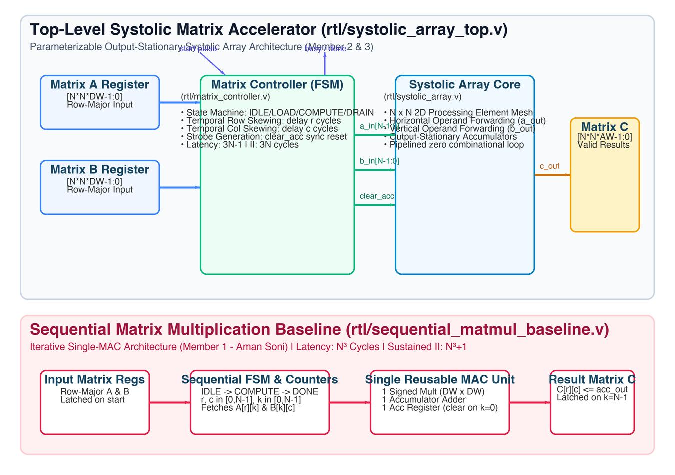
\includegraphics[width=0.92\textwidth]{figures/fig_a_system_block}
\caption{Top-level architectural block diagram comparing the scalable parameterizable systolic array accelerator (top) and the single-MAC sequential reference baseline (bottom).}
\label{fig:system_block}
\end{figure*}

\subsection{Processing Element Architecture}
The Processing Element (\texttt{rtl/processing\_element.v}) forms the foundational arithmetic unit of the accelerator. It is parameterized by operand bit-width (\texttt{DATA\_WIDTH}) and accumulator bit-width (\texttt{ACC\_WIDTH}), subject to the requirement $\text{ACC\_WIDTH} \ge 2 \times \text{DATA\_WIDTH}$. The internal datapath and register organization of the Processing Element are shown in Fig.~\ref{fig:pe_datapath}.

\begin{figure}[!t]
\centering
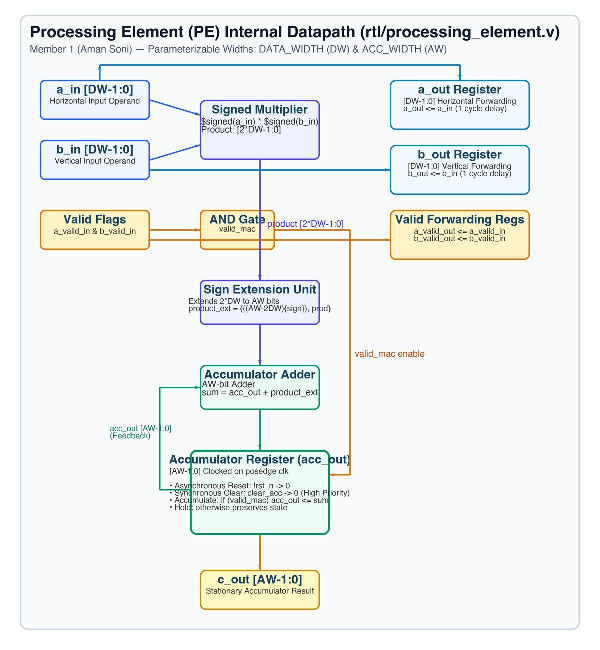
\includegraphics[width=\columnwidth]{figures/fig_b_pe_datapath}
\caption{Processing Element (PE) internal datapath showing signed multiplier, sign-extension unit, accumulator register with priority synchronous clear, and spatial forwarding registers.}
\label{fig:pe_datapath}
\end{figure}

The PE contains:
\begin{enumerate}
    \item \textbf{Signed Multiplier:} Multiplies signed operands \texttt{a\_in} and \texttt{b\_in} combinationally:
    \begin{equation}
    \text{product} = a_{\text{in}} \times b_{\text{in}}
    \end{equation}
    producing a signed intermediate product of $2 \times \text{DATA\_WIDTH}$ bits.
    \item \textbf{Sign-Extension Unit:} When $\text{ACC\_WIDTH} > 2 \times \text{DATA\_WIDTH}$, the product is sign-extended to \texttt{ACC\_WIDTH} bits by replicating its most significant bit ($p_{\text{msb}}$):
    \begin{equation}
    \text{product\_ext} = \big\{\{E\{p_{\text{msb}}\}\}, \, \text{product}\big\}
    \end{equation}
    where $E = \text{ACC\_WIDTH} - 2\cdot\text{DATA\_WIDTH}$ is the extension bit-width.
    \item \textbf{Accumulator Register:} On the rising clock edge with active-low asynchronous reset (\texttt{rst\_n}), all internal registers are cleared. Synchronous accumulator clearing (\texttt{clear\_acc}) takes highest priority, resetting \texttt{acc\_out} to zero. When \texttt{clear\_acc} is deasserted and both \texttt{a\_valid\_in} and \texttt{b\_valid\_in} are asserted, the product is accumulated:
    \begin{equation}
    \text{acc\_out} \Leftarrow \text{acc\_out} + \text{product\_ext}
    \end{equation}
    If either valid signal is deasserted, the accumulator preserves its value.
    \item \textbf{Spatial Forwarding Registers:} On each rising clock edge, operands and valid flags are registered and forwarded to neighboring PEs:
    \begin{align}
    a_{\text{out}} &\Leftarrow a_{\text{in}}, & b_{\text{out}} &\Leftarrow b_{\text{in}} \\
    a_{\text{valid\_out}} &\Leftarrow a_{\text{valid\_in}}, & b_{\text{valid\_out}} &\Leftarrow b_{\text{valid\_in}}
    \end{align}
    enabling pipelined systolic communication without combinational loops.
\end{enumerate}

\subsection{Scalable Systolic Array Core}
The systolic array module (\texttt{rtl/systolic\_array.v}) instantiates an $N \times N$ grid of PEs using nested Verilog \texttt{generate} constructs. Input operands for row $r$ and column $c$ must arrive at PE($r, c$) with relative temporal skew: an operand corresponding to common index $k$ arrives at PE($r, c$) on sampling clock edge $k + r + c$.

Fig.~\ref{fig:array_mesh} illustrates the interconnected $4 \times 4$ PE mesh, depicting the horizontal streaming of Matrix A, vertical streaming of Matrix B, and local accumulation of stationary partial sums within each PE.

\begin{figure}[!t]
\centering
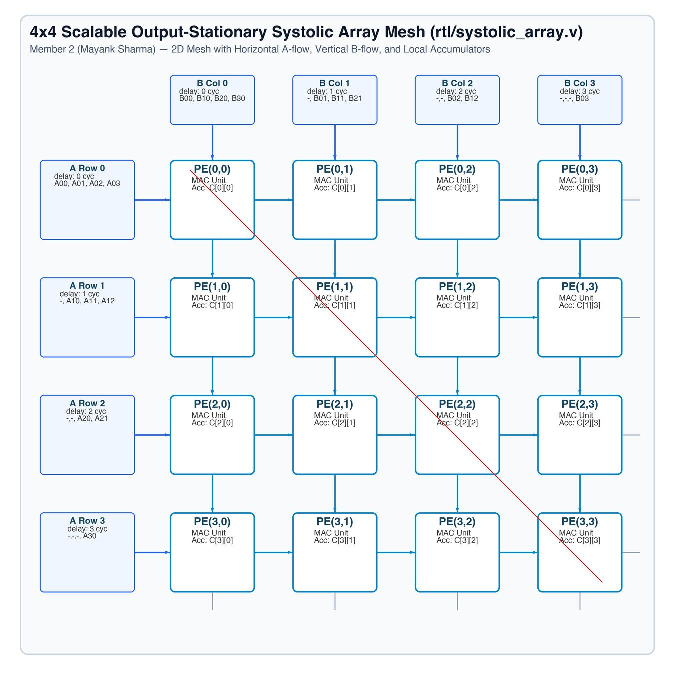
\includegraphics[width=\columnwidth]{figures/fig_c_array_mesh}
\caption{A $4 \times 4$ output-stationary systolic array mesh illustrating horizontal operand forwarding for Matrix A, vertical operand forwarding for Matrix B, and local accumulation of partial sums.}
\label{fig:array_mesh}
\end{figure}

To present a natural row-major matrix interface to external logic, the array core incorporates integrated input skewing buffers. Row lane $r$ is delayed by $r$ clock cycles using an $r$-stage register pipeline, and column lane $c$ is delayed by $c$ clock cycles using a $c$-stage register pipeline. The first lane ($r=0, c=0$) connects directly without delay. At the completion of accumulation, all $N^2$ local accumulators are mapped to a single concatenated output bus.

\subsection{Matrix Controller and Execution Schedule}
The matrix controller (\texttt{rtl/matrix\_controller.v}) governs the accelerator handshake and execution schedule. The cycle-by-cycle execution schedule governed by the controller FSM is diagrammed in Fig.~\ref{fig:controller_schedule} for an $N=4$ configuration.

\begin{figure}[!t]
\centering
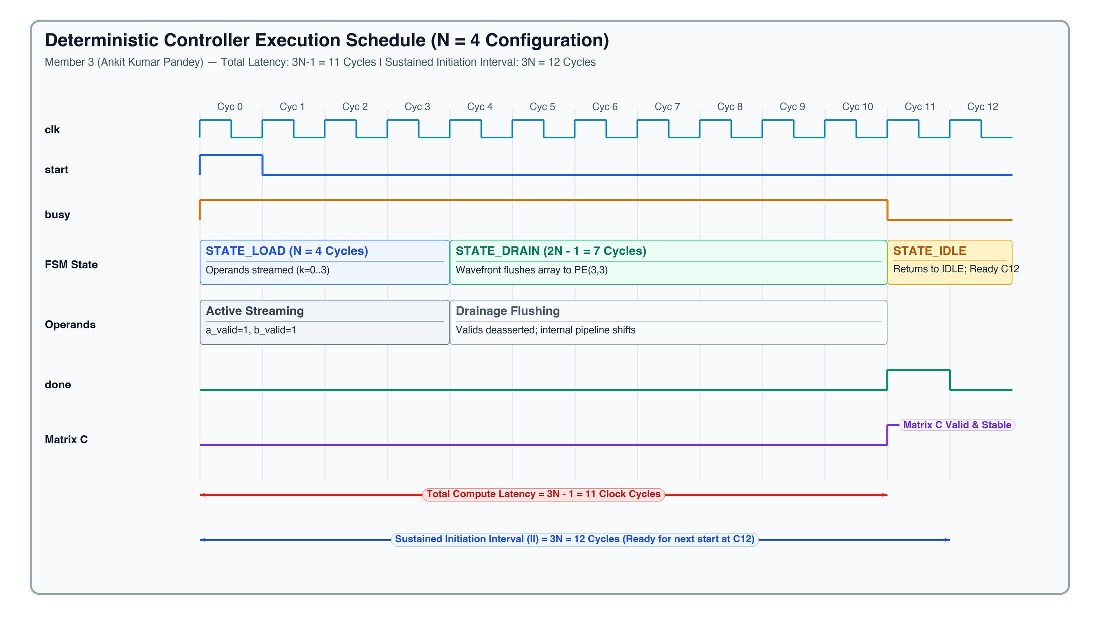
\includegraphics[width=\columnwidth]{figures/fig_d_controller_schedule}
\caption{Deterministic execution schedule for an $N=4$ configuration, detailing the $N$-cycle loading phase, $(2N-1)$-cycle draining phase, total compute latency of $3N-1 = 11$ clock cycles, and initiation interval of $3N = 12$ cycles.}
\label{fig:controller_schedule}
\end{figure}

The controller coordinates a three-state finite state machine:
\begin{enumerate}
    \item \texttt{STATE\_IDLE} (\texttt{2'd0}): The controller asserts \texttt{busy=0} and \texttt{done=0}. When \texttt{start} is asserted, the controller latches the external matrix buses \texttt{a\_flat} and \texttt{b\_flat} into internal registers \texttt{a\_latched} and \texttt{b\_latched}. Concurrently, \texttt{clear\_acc} is combinationally asserted to initialize all array accumulators, \texttt{busy} is set to 1, and the FSM transitions to \texttt{STATE\_LOAD}.
    \item \texttt{STATE\_LOAD} (\texttt{2'd1}): The controller streams $k$-slices ($k = 0, \dots, N-1$) of the latched matrices into the array lanes across $N$ consecutive clock cycles. Slicing logic drives row lane $r$ with $A[r][k]$ and column lane $c$ with $B[k][c]$, asserting \texttt{a\_valid} and \texttt{b\_valid}. Once $k = N-1$, the FSM transitions to \texttt{STATE\_DRAIN}.
    \item \texttt{STATE\_DRAIN} (\texttt{2'd2}): Input valids are deasserted. Over $2N-1$ clock cycles, the final computational wavefront traverses the array to PE($N-1, N-1$). On the final cycle, \texttt{result} latches the completed accumulator values from the array, \texttt{busy} drops to 0, \texttt{done} asserts as a single-cycle pulse, and the FSM returns to \texttt{STATE\_IDLE}.
\end{enumerate}

The total measured latency from \texttt{start} acceptance to \texttt{done} assertion is:
\begin{equation}
L_{\text{systolic}} = 3N - 1 \quad \text{cycles}
\end{equation}
The sustained initiation interval (II) between back-to-back operations is:
\begin{equation}
\text{II}_{\text{systolic}} = 3N \quad \text{cycles}
\end{equation}
where the additional cycle corresponds to returning to \texttt{STATE\_IDLE} before accepting the next \texttt{start} request.

\subsection{Top-Level Accelerator Module}
The top-level module (\texttt{rtl/systolic\_array\_top.v}) structurally integrates the matrix controller and systolic array into a self-contained accelerator. Input matrices and results are exchanged over flattened row-major buses:
\begin{itemize}
    \item Input matrix $A$ or $B$ width: $N \times N \times \text{DATA\_WIDTH}$ bits. An element at row $r$ and column $c$ occupies slice $\text{matrix}[\text{idx}_{\text{in}} +: \text{DATA\_WIDTH}]$, where:
    \begin{equation}
    \text{idx}_{\text{in}} = (r \cdot N + c) \cdot \text{DATA\_WIDTH}
    \end{equation}
    \item Output matrix $C$ width: $N \times N \times \text{ACC\_WIDTH}$ bits. An accumulated element at row $r$ and column $c$ occupies slice $\text{result}[\text{idx}_{\text{out}} +: \text{ACC\_WIDTH}]$, where:
    \begin{equation}
    \text{idx}_{\text{out}} = (r \cdot N + c) \cdot \text{ACC\_WIDTH}
    \end{equation}
\end{itemize}

\subsection{Sequential Matrix Multiplication Baseline}
To quantify the acceleration benefits of spatial systolic parallelism, a hardware sequential baseline (\texttt{rtl/sequential\_matmul\_baseline.v}) was developed using the exact same top-level interface. The baseline accelerator implements a single shared MAC unit and a sequential control engine with counters $r\_cnt$, $c\_cnt$, and $k\_cnt$.

Upon receiving \texttt{start}, the baseline latches the input matrices and iterates through the standard triple loop:
\begin{equation}
C[r][c] = \sum_{k=0}^{N-1} A[r][k] \times B[k][c]
\end{equation}
Executing one MAC operation per clock cycle, the baseline requires:
\begin{equation}
L_{\text{seq}} = N^3 \quad \text{cycles}
\end{equation}
Its sustained initiation interval is $\text{II}_{\text{seq}} = N^3 + 1$ cycles.

Table~\ref{tab:baseline_2x2_trace} provides the hand-verified cycle-by-cycle execution trace of a $2 \times 2$ matrix multiplication on the sequential baseline, demonstrating the exact 8-cycle computation for $A = \begin{pmatrix} 1 & 2 \\ 3 & 4 \end{pmatrix}$ and $B = \begin{pmatrix} 5 & 6 \\ 7 & 8 \end{pmatrix}$ producing $C = \begin{pmatrix} 19 & 22 \\ 43 & 50 \end{pmatrix}$ with $N^3 = 8$ cycles.

\begin{table}[htbp]
\caption{Cycle-by-Cycle Execution Trace for $2 \times 2$ Matrix Multiplication on Sequential Baseline}
\label{tab:baseline_2x2_trace}
\centering
\setlength{\tabcolsep}{4.5pt}
\begin{tabular}{cccccccc}
\toprule
Cycle & $r$ & $c$ & $k$ & $A[r][k]$ & $B[k][c]$ & Product & Accumulator / Output \\
\midrule
1 & 0 & 0 & 0 & 1 & 5 & 5  & 5 \\
2 & 0 & 0 & 1 & 2 & 7 & 14 & $19 \implies C[0][0]=19$ \\
3 & 0 & 1 & 0 & 1 & 6 & 6  & 6 \\
4 & 0 & 1 & 1 & 2 & 8 & 16 & $22 \implies C[0][1]=22$ \\
5 & 1 & 0 & 0 & 3 & 5 & 15 & 15 \\
6 & 1 & 0 & 1 & 4 & 7 & 28 & $43 \implies C[1][0]=43$ \\
7 & 1 & 1 & 0 & 3 & 6 & 18 & 18 \\
8 & 1 & 1 & 1 & 4 & 8 & 32 & $50 \implies C[1][1]=50$ \\
\bottomrule
\end{tabular}
\end{table}

\section{Results and Discussion}

\subsection{Experimental Methodology}
All hardware verification and performance measurements were conducted using Icarus Verilog and Python 3.14 on macOS (Apple silicon). Simulations are cycle-accurate and evaluate full register transfers, state transitions, and bus handshakes. Performance metrics assume a system clock frequency of 100~MHz (10~ns clock period).

\begin{quote}
\textit{Clarification of Evaluation Scope:} All reported numbers represent cycle-accurate RTL logic simulation results. No FPGA synthesis, place-and-route, post-fit timing, physical silicon area, or hardware resource utilization (LUT, flip-flop, DSP, or BRAM counts) was measured.
\end{quote}

\subsection{Performance Comparison Across Configurations}
Table~\ref{tab:system_results} details the measured latency, throughput, and speedup metrics across nine distinct architectural configurations, extracted directly from the system benchmark summary (\texttt{sim/results/system\_summary.csv}).

\begin{table*}[t]
\caption{Measured Performance Comparison of Systolic Accelerator vs. Sequential Baseline}
\label{tab:system_results}
\centering
\setlength{\tabcolsep}{4.5pt}
\begin{tabular}{cccrrrrrrr}
\toprule
$N$ & \texttt{DATA\_WIDTH} & \texttt{ACC\_WIDTH} & \begin{tabular}{@{}c@{}}Systolic Lat.\\(cycles)\end{tabular} & \begin{tabular}{@{}c@{}}Seq. Lat.\\(cycles)\end{tabular} & \begin{tabular}{@{}c@{}}Latency\\Speedup\end{tabular} & \begin{tabular}{@{}c@{}}Systolic II\\(cycles)\end{tabular} & \begin{tabular}{@{}c@{}}Seq. II\\(cycles)\end{tabular} & \begin{tabular}{@{}c@{}}Throughput\\Speedup\end{tabular} & Status \\
\midrule
1 & 8  & 32 & 2  & 1   & $0.50\times$  & 3  & 2   & $0.67\times$  & PASS \\
2 & 8  & 32 & 5  & 8   & $1.60\times$  & 6  & 9   & $1.50\times$  & PASS \\
3 & 8  & 32 & 8  & 27  & $3.38\times$  & 9  & 28  & $3.11\times$  & PASS \\
4 & 8  & 32 & 11 & 64  & $5.82\times$  & 12 & 65  & $5.42\times$  & PASS \\
8 & 8  & 32 & 23 & 512 & $22.26\times$ & 24 & 513 & $21.38\times$ & PASS \\
2 & 16 & 32 & 5  & 8   & $1.60\times$  & 6  & 9   & $1.50\times$  & PASS \\
4 & 16 & 48 & 11 & 64  & $5.82\times$  & 12 & 65  & $5.42\times$  & PASS \\
4 & 8  & 16 & 11 & 64  & $5.82\times$  & 12 & 65  & $5.42\times$  & PASS \\
8 & 16 & 48 & 23 & 512 & $22.26\times$ & 24 & 513 & $21.38\times$ & PASS \\
\bottomrule
\end{tabular}
\end{table*}

Fig.~\ref{fig:pe_waveform} illustrates the simulation timing waveform extracted directly from \texttt{sim/waveforms/pe\_8bit.vcd} for Test~1 ($3 \times 4 = 12$), confirming the strict one-cycle spatial operand forwarding delay between \texttt{a\_in} and \texttt{a\_out}.

\begin{figure}[!t]
\centering
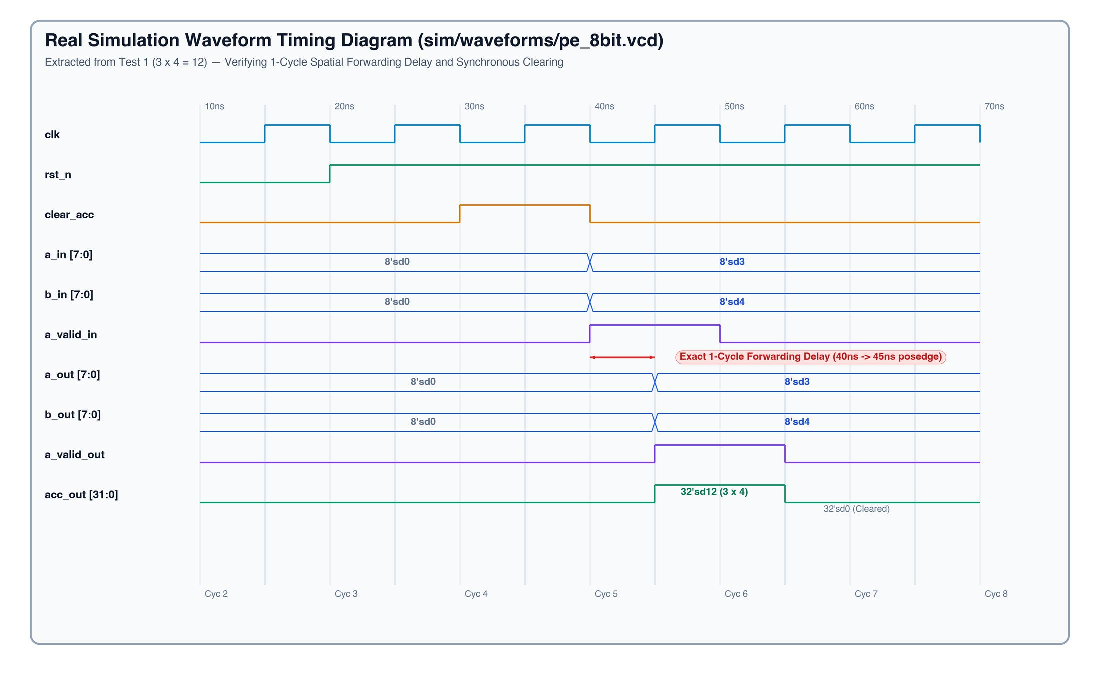
\includegraphics[width=\columnwidth]{figures/fig_e_pe_waveform}
\caption{Simulation timing waveform extracted directly from \texttt{sim/waveforms/pe\_8bit.vcd} during Test~1 ($3 \times 4 = 12$), confirming the strict one-cycle spatial operand forwarding delay between \texttt{a\_in} and \texttt{a\_out} alongside synchronous accumulator clearing and valid gating.}
\label{fig:pe_waveform}
\end{figure}

\subsection{Analytical Scaling and Latency Discussion}
The empirical results confirm the theoretical complexity models:
\begin{enumerate}
    \item \textbf{Algorithmic Scaling:} While the single-MAC sequential baseline scales cubically as $\mathcal{O}(N^3)$ (requiring 8, 64, and 512 cycles for $N=2, 4,$ and $8$), the systolic array scales linearly as $\mathcal{O}(N)$ ($3N-1$ cycles, yielding 5, 11, and 23 cycles). Consequently, the latency speedup scales approximately as $\mathcal{O}(N^2 / 3)$, reaching $5.82\times$ at $N=4$ and $22.26\times$ at $N=8$. Fig.~\ref{fig:latency_scaling} plots the measured execution latencies on a logarithmic scale, validating the linear scaling $\mathcal{O}(N)$ of the systolic array ($3N-1$ cycles) against the cubic $\mathcal{O}(N^3)$ growth of the sequential baseline.
    \item \textbf{Sustained Throughput and Speedup:} Sustained throughput grows with array dimension, operating at $N^3 / (3N) = N^2 / 3$ MACs per cycle on the systolic array versus approximately 1 MAC per cycle on the baseline. At $N=8$ and 100~MHz, the systolic array achieves 2,133.33~MMAC/s compared to 99.81~MMAC/s for the sequential engine ($21.38\times$ throughput speedup). Fig.~\ref{fig:speedup} details the resulting latency speedup across matrix dimensions, illustrating the crossover at $N \ge 2$ and the $22.26\times$ speedup at $N=8$.
    \item \textbf{Crossover Threshold:} At $N=1$, controller setup and draining overhead ($3N-1 = 2$ cycles) exceeds the single MAC calculation of the baseline (1 cycle), resulting in a speedup of $0.50\times$. For all dimensions $N \ge 2$, the systolic architecture decisively outperforms the sequential design.
    \item \textbf{Controller Evolution (Phase I vs. Phase II):} In Phase I of the project, a fixed 4$\times$4 design exhibited a 14-cycle compute latency. That schedule allocated 1 cycle for dedicated state clearing (\texttt{STATE\_CLEAR}), 4 cycles for loading, 8 cycles for draining, and 1 cycle for registered output latching ($1 + 4 + 8 + 1 = 14$). In Phase II, the parameterized controller was re-architected to assert \texttt{clear\_acc} combinationally upon detecting \texttt{start} in \texttt{STATE\_IDLE}, simultaneously latching input operands. The compute wavefront begins streaming immediately on the subsequent clock edge, compressing total latency to $3N-1$ cycles (11 cycles for $N=4$).
    \item \textbf{Precision Independence:} Configurations with extended 16-bit operands (\texttt{DATA\_WIDTH=16, ACC\_WIDTH=48}) and reduced accumulator width (\texttt{ACC\_WIDTH=16}) display identical cycle counts to the 8-bit baseline, confirming that the control path is completely decoupled from arithmetic bit-widths.
\end{enumerate}

\begin{figure}[!t]
\centering
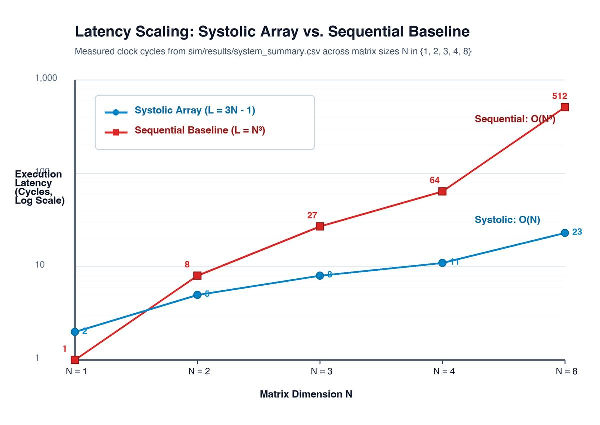
\includegraphics[width=\columnwidth]{figures/fig_f_latency_scaling}
\caption{Measured latency scaling comparing the systolic array ($3N-1$ cycles, $\mathcal{O}(N)$) against the sequential baseline ($N^3$ cycles, $\mathcal{O}(N^3)$) across matrix dimensions $N \in \{1, 2, 3, 4, 8\}$ on a logarithmic scale.}
\label{fig:latency_scaling}
\end{figure}

\begin{figure}[!t]
\centering
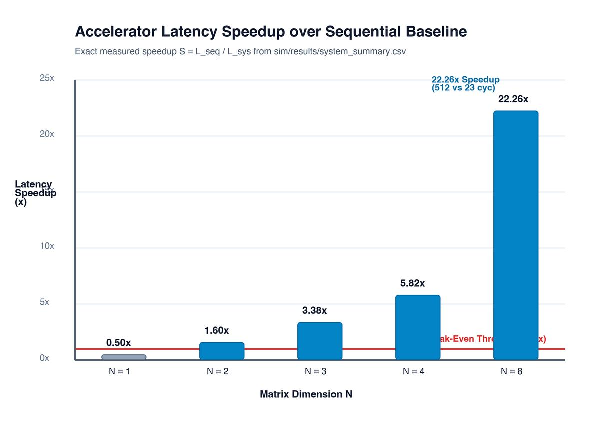
\includegraphics[width=\columnwidth]{figures/fig_g_speedup}
\caption{Measured latency speedup of the systolic accelerator over the sequential baseline across matrix sizes $N \in \{1, 2, 3, 4, 8\}$, highlighting the $1.0\times$ break-even threshold and peak speedup of $22.26\times$ at $N=8$.}
\label{fig:speedup}
\end{figure}

\subsection{Comprehensive Verification Summary}
The hardware was validated across four verification suites:
\begin{itemize}
    \item \textbf{Processing Element Unit Testbench (\texttt{tb\_processing\_element.v}):} 14 directed test cases verifying positive, negative, and mixed-sign multiplication, zero operand handling, multi-cycle accumulation, invalid operand gating, clear priority over simultaneous multiplication, reset clearing, data forwarding, signed extreme boundary conditions, and accumulator two's complement wraparound (131,073 continuous accumulations of $(-128) \times (-128) = 16,384$ wrapping to $-2,147,467,264$ in 32-bit signed representation). All 14 tests passed in both 8-bit/32-bit and 16-bit/48-bit configurations.
    \item \textbf{Array Core Scoreboard (\texttt{tb\_systolic\_array\_core.v}):} Evaluated across 10 configurations (including non-power-of-two grids such as $3 \times 3$), testing 110 matrices and 1,838 clock edges per configuration against a cycle-accurate software scoreboard. All 10 configurations passed with zero errors.
    \item \textbf{System Integration Regression (\texttt{tb\_systolic\_array.v}):} Evaluated across 9 parameter configurations covering 46 test cases per configuration (8 directed cases, 31 golden-model vectors, 4 randomized cases, bus corrupt-immunity tests, back-to-back throughput tests, and mid-compute reset recovery), totaling 414 test cases. All 414 cases passed with zero mismatches.
    \item \textbf{Golden Model Unit Suite (\texttt{test\_golden\_model.py}):} 12 unit tests verifying bit-level packing, signed overflow modulo $2^{\text{ACC\_WIDTH}}$, vector file round-tripping, and mathematical equivalence against naive matrix multiplication. All 12 tests passed.
\end{itemize}

Fig.~\ref{fig:verification_summary} summarizes the complete multi-tier test suite, demonstrating 100\% pass rates across all 476 automated test vectors.

\begin{figure}[!t]
\centering
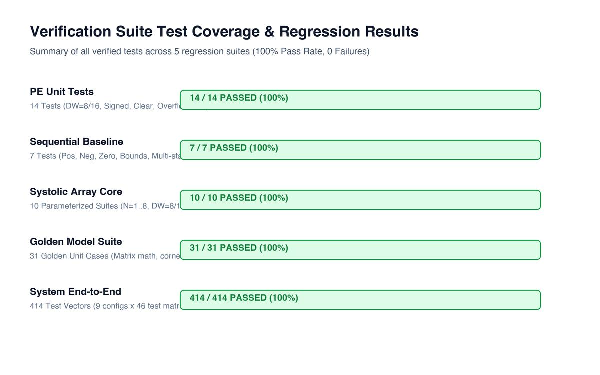
\includegraphics[width=\columnwidth]{figures/fig_h_verification_summary}
\caption{Summary of verification test coverage and pass rates across all five regression suites, demonstrating a 100\% pass rate across 476 automated test vectors with zero functional mismatches.}
\label{fig:verification_summary}
\end{figure}

\section{Individual Contributions}
The project workload and module ownership were distributed among the three team members as follows:

\begin{itemize}
    \item \textbf{Member 1 --- Aman Soni (Processing Element Design \& Sequential Baseline):}
    \begin{itemize}
        \item Designed and implemented the parameterizable Processing Element module in Verilog (\texttt{rtl/processing\_element.v}) with signed multiplication, parameter-driven sign extension, synchronous accumulator clearing priority, and data/valid forwarding.
        \item Designed and implemented the parameterizable sequential matrix multiplication baseline engine (\texttt{rtl/sequential\_matmul\_baseline.v}) with single-MAC datapath, multi-state control, and row-major bus parsing.
        \item Developed unit testbenches (\texttt{testbench/tb\_processing\_element.v} and \texttt{testbench/tb\_sequential\_baseline.v}), implementing 14 comprehensive PE test scenarios (including signed boundary tests and accumulator overflow wraparound verification) and multi-size baseline verification.
        \item Authored the architectural Phase II Interface Contract defining unified parameter semantics and row-major bus slicing conventions.
    \end{itemize}

    \item \textbf{Member 2 --- Mayank Sharma (Systolic Array Mesh \& Core Verification):}
    \begin{itemize}
        \item Designed and implemented the scalable 2D systolic array core (\texttt{rtl/systolic\_array.v}) using nested generate loops to instantiate an $N \times N$ PE grid.
        \item Implemented the parameterizable integrated input skewing register stages, establishing spatial diagonal delay alignment for arbitrary array dimensions.
        \item Connected horizontal and vertical operand forwarding paths and mapped internal PE accumulators to the wide parallel output bus.
        \item Developed the cycle-by-cycle array core verification scoreboard (\texttt{testbench/tb\_systolic\_array\_core.v}) and regression automation script (\texttt{verification/run\_array\_tests.py}), verifying 10 distinct architectural geometries.
    \end{itemize}

    \item \textbf{Member 3 --- Ankit Kumar Pandey (Matrix Controller, Top Level, \& System Benchmarking):}
    \begin{itemize}
        \item Designed and implemented the parameterizable FSM matrix controller (\texttt{rtl/matrix\_controller.v}) featuring input operand latching, start/busy/done handshaking, and the optimal $3N-1$ LOAD/DRAIN execution schedule.
        \item Implemented the unified top-level structural wrapper (\texttt{rtl/systolic\_array\_top.v}).
        \item Implemented the bit-accurate Python golden model and vector generator (\texttt{verification/golden\_model.py}) and comprehensive golden unit test suite (\texttt{verification/test\_golden\_model.py}).
        \item Developed the end-to-end integration testbench (\texttt{testbench/tb\_systolic\_array.v}) and multi-configuration regression suite (\texttt{verification/run\_system\_tests.py}), executing 414 test cases and compiling the empirical performance benchmark.
    \end{itemize}
\end{itemize}

\section{Conclusion}
This project successfully designed, implemented, and verified a parameterizable output-stationary systolic array matrix multiplication accelerator alongside a single-MAC sequential baseline in Verilog HDL. By integrating input skewing buffers and a deterministic FSM controller, the accelerator computes an $N \times N$ matrix product in exactly $3N-1$ clock cycles. Cycle-accurate simulation across nine configurations validated arithmetic equivalence against a Python golden model across 414 test cases with zero errors. Comparative analysis proved that the systolic architecture scales as $\mathcal{O}(N)$ compute latency, achieving a $22.26\times$ latency speedup and $21.38\times$ sustained throughput improvement over the sequential baseline for $8 \times 8$ matrix operations.

\begin{thebibliography}{0}
\bibitem{kung1978} H. T. Kung and C. E. Leiserson, ``Systolic arrays (for VLSI),'' in \textit{Sparse Matrix Proceedings 1978}, I. S. Duff and G. W. Stewart, Eds. Philadelphia, PA, USA: SIAM, 1979, pp. 256--282. [Online]. Available: \url{https://apps.dtic.mil/sti/tr/pdf/ADA067674.pdf}
\bibitem{jouppi2017} N. P. Jouppi et al., ``In-datacenter performance analysis of a tensor processing unit,'' in \textit{Proc. 44th Annu. Int. Symp. Comput. Archit. (ISCA)}, Toronto, ON, Canada, Jun. 2017, pp. 1--12. [Online]. Available: \url{https://doi.org/10.1145/3079856.3080246}
\bibitem{patterson2020} D. A. Patterson and J. L. Hennessy, \textit{Computer Organization and Design RISC-V Edition: The Hardware/Software Interface}, 2nd ed. San Francisco, CA, USA: Morgan Kaufmann, 2020, ch. 4--6. [Online]. Available: \url{https://www.elsevier.com/books/computer-organization-and-design-risc-v-edition/patterson/978-0-12-812275-4}
\end{thebibliography}

\end{document}
